\chapter{Простой пример нагруженного <<толстого>> цилиндра} \label{ch:example1}

Рассмотрим вот такой пример...
Допустим, есть толстостенные цилиндр с внотренними и внешними радиусами \(a=1\,m\) и \(b=1.2\,m\) и высотой \(l~=~1\,m\). Коэффициент Пуассона \(\mu=0.3\) и модуль упругости и коэффициент термального расширения на внутреннем радиусе \(E_i = 200\,Gpa\) и \(\alpha_i = 1.2 \times 10^{-6} /^{\circ}C\) задаются уравнением \cref{eq:ch2:equation4} и коэффициент теплопроводности записывается в таком же виде \( k(r) = k_0 \big ( \frac{r}{l} \big ) ^ {m_3} \) (в самом общем случае напряжения выжараются тоже степенной функцией в следующем виде \(\sigma_y(r) = \sigma_0 (\frac{r}{l})^{m_4}\)). Для простоты степенная функция распределения свойст материалов будет одинаковым \(m_1=m_2=m_3=m\).

На внутренней границе отсутсвует сила, только задана температура по следующему закону (\(T = T(r, \phi)\)):
\begin{equation}
\label{eq:example1:1}
\begin{split}
	T(a, \phi) &= 60 cos (3\phi^{\circ}C) \\
	T(b, \phi) &= 0
\end{split}
\end{equation}
 --- не осесимметричное нагружение. Внешняя граница закреплена --- запрещены перемещения в радиальном направлении с нулевой температурой. 
\begin{equation}
\label{eq:example1:2}
\begin{split}
	\sigma_{rr}(a, \phi) &= 0,\\
	\sigma_{r\phi}(a, \phi) &= 0,\\
	u(b, \phi) &= 0,\\
	v(b, \phi) &= 0
\end{split}
\end{equation}

Чтобы получить температурное распределение, как \cref{eq:ch2:equation6}, определеним константы интегрирования \(A_1, A_2\) подставив температуру в дифференциальное уравнение теплопроводности (в цилиндрической СК).

\begin{equation}
	\label{eq:example1:3}
	\frac{1}{r} \frac{\partial}{\partial r} \left (k r \frac{\partial T}{\partial r} \right) + \frac{1}{r^2} \frac{\partial}{\partial \theta} \left (k \frac{\partial T}{\partial \theta} \right ) + \frac{\partial}{\partial z} \left (k \frac{\partial T}{\partial z} \right) + R = \rho c \frac{\partial T}{\partial t}
\end{equation}





Что в случае отсутсвия источников тепла, нагружения (правой части) и оси симметрии выразится в следующем уравнении, а также зависимоти температуры только от окружного расположения. Рассматриваем полностью установившееся равновесие:

\begin{equation}
	\label{eq:example1:4}
	\frac{1}{r} \frac{\partial}{\partial r} \left (k(r) r \frac{\partial T}{\partial r} \right) + \frac{1}{r^2} \frac{\partial}{\partial \theta} \left (k(r) \frac{\partial T}{\partial \theta} \right ) = 0
\end{equation}

Упрощая

\begin{equation*}
	\frac{1}{r} \frac{\partial}{\partial r} \left (k(r) r \frac{\partial T}{\partial r} \right) + \frac{k(r)}{r^2}  \frac{\partial^2 T}{\partial \theta^2} = 0
\end{equation*}

Получими уравнение теплопроводности для установившегося состояния 2д случая в полярной СК и с граничными условиями для ФГМ шилиндра ниже:
\begin{equation}
	\label{eq:example1:5}
	\frac{\partial^2 T}{\partial r^2} + \left ( \frac{ k^{\prime}(r)}{k(r)} + \frac{1}{r} \right )\frac{\partial T}{\partial r} + \frac{1}{r^2}\frac{\partial^2 T}{\partial \theta^2} = 0 \quad a \le r \le b \quad -\pi \le \phi \le \pi
\end{equation}

\begin{equation}
	\label{eq:example1:6}
	\begin{split}
		C_{11} T(a, \phi) + C_{12} T_{,r}(a, \phi) = f_1 (\phi)& = 60 cos{3 \phi} \\
		C_{21} \xcancel{T(b, \phi)} + C_{22} \xcancel{T_{,r}(b, \phi)} &= \cancel{f_2 (\phi)}
	\end{split}
\end{equation}
где \(C_{ij}\) постоянные термические параметры связанные с теплопроводностью и коэффициентами конвекции, а \(f_i(\phi)\) известные функции распределения температуры на радиусах цилиндра.

Подставим \(k(r)\) в уравнение \cref{eq:example1:5}) и получим следующее


\begin{equation}
	\label{eq:example1:7}
	T_{,rr} + (m+1)\frac{1}{r}T_{,r}+\frac{1}{r^2}T_{,\phi \phi} =0
\end{equation}

Так как функция \(T(r, \phi)\) переодическая, то можно найти решение в виде комплексного ряда Фурье
\begin{equation}
	\label{eq:example1:8}
	T(r, \phi) = \sum_{n=-\infty}^{\infty} T_{n}(r) e^{in\phi}
\end{equation}
где коэффициент Т на конечной комплексной плоскости определяется

\begin{equation}
	\label{eq:example1:9}
	T_n(r) = \frac{1}{2\pi} \int_{-\pi}^{\pi} T(r, \phi) e^{-in\phi} \,d\phi
\end{equation}

Подставляя \cref{eq:example1:9} \cref{eq:example1:7}

\begin{equation}
	\label{eq:example1:10}
	T_{n}^{\prime \prime} + (m+1)\frac{1}{r}T_{n}^{\prime}-\frac{n^2}{r^2}T_{n} =0
\end{equation}

Решение этого уравнения находится в виде \(T_n(r) = A_n r^{\beta}\), которое после подстановки в предыдущее уравнение дает следующее квадратичное уравнение с корнями

\begin{equation*}
	\begin{split}
		\beta^2 +m \beta - n^2 =0\\
		\beta_{n1,2} = -\frac{m}{2} \pm \left(\frac{m^2}{4} + n^2 \right)^{\frac{1}{2}}
	\end{split}
\end{equation*}
или
при \(n=0, n=1, m=4\)


что с последующей подстановкой приводит к решению в общем виде

\begin{equation*}
	T_n(r) = A_{n1} r^{\beta_{n1}} + A_{n2} r^{\beta_{n2}}
\end{equation*}

\begin{equation}
	\label{eq:example1:11}
	T(r, \phi) = \sum_{n=-\infty}^{\infty} \left ( A_{n1} r^{\beta_{n1}} + A_{n2} r^{\beta_{n2}} \right ) e^{in\phi}
\end{equation}



Для нахождение коэффициентов А, подставим рещение в ГУ \cref{eq:example1:6}

\begin{equation*}
\begin{split}
\sum_{n=-\infty}^{\infty} \left [ \left (C_{11} a^{\beta_{n1}} +C_{12} \beta_{n1} a^{\beta_{n1} -1} \right ) A_{n1}  +\left (C_{11} a^{\beta_{n2}} +C_{12} \beta_{n2} a^{\beta_{n2} -1} \right ) A_{n2} \right ] e^{in\phi} = f_1(\phi) \\
\sum_{n=-\infty}^{\infty} \left [ \left (C_{21} b^{\beta_{n1}} +C_{22} \beta_{n1} a^{\beta_{n1} -1} \right ) A_{n1}  +\left (C_{21} b^{\beta_{n2}} +C_{22} \beta_{n2} b^{\beta_{n2} -1} \right ) A_{n2} \right ] e^{in\phi} = f_2(\phi)
\end{split}
\end{equation*}


%сравнить с примером из этой статьи Dinkar Sharma* and Ramandeep Kaur
% Thermoelastic analysis of FGM hollow cylinder for
% variable parameters and temperature
% distributions using FEM
{\color{red}
Вот тут будет продолжение примера. Пока возникли проблемы с реализацией, но должно оплучиться что-то в таком виде.
В запасе есть еще пример с другими ГУ
}
\begin{figure}[ht]
	\begin{minipage}[h]{.4\textwidth}
		\centering
		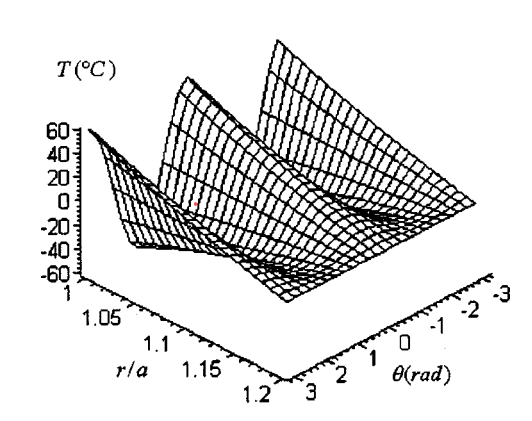
\includegraphics[width=1\textwidth]{example1_fig1.png}
		\caption{Распределение температуры по толщине. К этому я стремлюсь}
	\end{minipage}
	\hfill
	\begin{minipage}[h]{.4\textwidth}
		\centering
		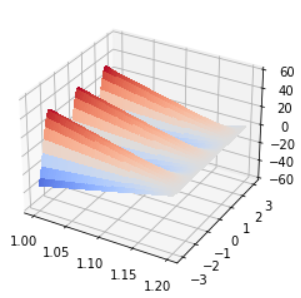
\includegraphics[width=1\textwidth]{example1_fig1b.png}
		\caption{Распределение температуры по толщине. Пока выходит так}
	\end{minipage}
\end{figure}

\begin{figure}[ht]
	\begin{minipage}[h]{.4\textwidth}
		\centering
		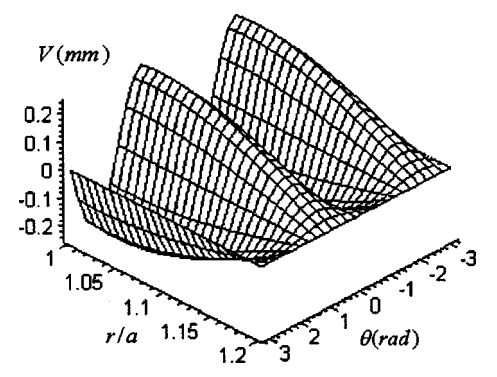
\includegraphics[width=1\textwidth]{example1_fig2.png}
		\caption{Радиальное перемещение по толщине}
	\end{minipage}
	\hfill
	\begin{minipage}[h]{.4\textwidth}
		\centering
		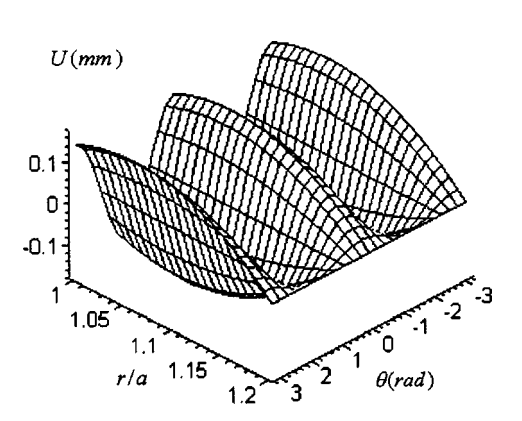
\includegraphics[width=1\textwidth]{example1_fig2a.png}
		\caption{Окружное перемещение по толщине}
	\end{minipage}
\end{figure}

\begin{figure}[ht]
	\begin{minipage}[h]{.4\textwidth}
		\centering
		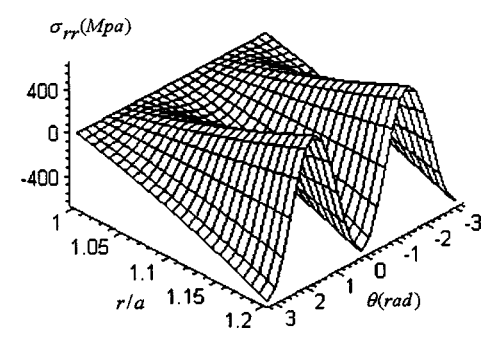
\includegraphics[width=1\textwidth]{example1_fig3a.png}
		\caption{Радиальное термальное напряжениепо толщине}
	\end{minipage}
	\hfill
	\begin{minipage}[h]{.4\textwidth}
		\centering
		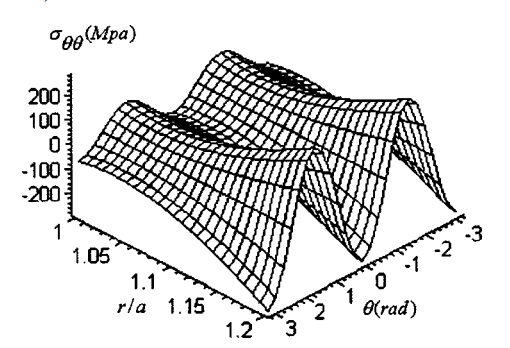
\includegraphics[width=1\textwidth]{example1_fig3b.png}
		\caption{Окружное термальное напряжениепо толщине}
	\end{minipage}
	\hfill
\begin{minipage}[h]{.4\textwidth}
	\centering
	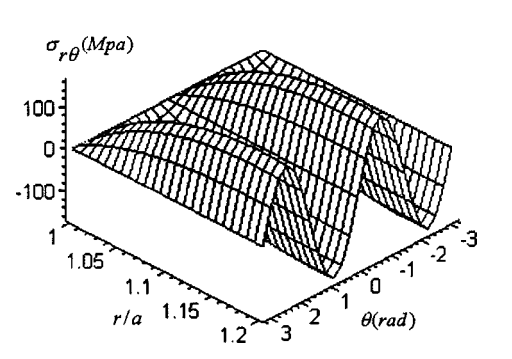
\includegraphics[width=1\textwidth]{example1_fig3c.png}
	\caption{Сдвиговое термальное напряжениепо толщине}
\end{minipage}
\end{figure}